\documentclass{article}
%% Chapter 2 Section 4: Adjoints

\usepackage{amsmath}
\usepackage{palatino}
\usepackage{tikz}

\newcommand{\one}{\mathbf{1}}
\newcommand{\cat}{\mathbf{C}}
\newcommand{\id}{\mathbf{id}}
\newcommand{\pifun}{\mathbf{\Pi}}
\newcommand{\diagfun}{\mathbf{\Delta}}

\begin{document}

\begin{enumerate}
\item [2.4.5]
  \begin{description}
  \item [Unit:]
    The unit diagram operates on the distinguised object $*$ of the category $\one$ and arbitrary objects $y$ of the category $\cat$.
    The functor $F : \one \rightarrow \cat$ is the left adjoint of the constant functor $T : \cat \rightarrow \one$ noted by Pierce.
    Additionally the unit $\iota : \id_\one \rightarrow \id_\one$ is fixed.
    \begin{center}
      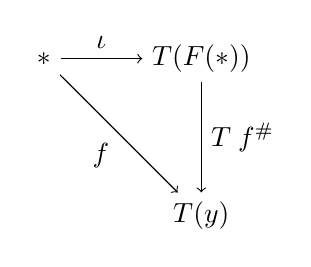
\begin{tikzpicture}
        \node (1) {$*$};
        \node [right of=1, xshift=1cm] (2) {$T(F(*))$};
        \node [below of=2, yshift=-1cm] (3) {$T(y)$};
        
        \draw[->] (1) -- node [above] {$\iota$} (2);
        \draw[->] (1) -- node[below left] {$f$} (3);
        \draw[->] (2) -- node [right] {$T~f^{\#}$} (3);
      \end{tikzpicture}
    \end{center}
    Looking back at the definition of an adjunction, we have that for each object of $\one$, each object of $\cat$, and each $\one$-arrow $f: X \rightarrow T(y)$ there is a unique $\cat$ arrow $f^{\#} : F(*) \rightarrow y$.
    Because there is only one object in the category $\one$, this definition says that for each object in $\cat$ there is a unique arrow $f^{\#}$ taking the image of the unique object of $\one$ to this object $y$.
    Thus the image of $*$ must be an initial object.

  \vfill{}
  \item [Co-unit:]
    Similarly, the counit diagram works in the opposite direction.
    \begin{center}
      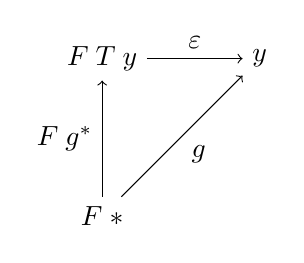
\begin{tikzpicture}
        \node (1) {$F~T~y$};
        \node [below of=1, yshift=-1cm] (2) {$F~*$};
        \node [right of=1, xshift=1cm] (3) {$y$};
        \draw[->] (2) -- node [left] {$F~g^*$} (1);
        \draw[->] (1) -- node[above] {$\varepsilon$} (3);
        \draw[->] (2) -- node [below right] {$g$} (3);
      \end{tikzpicture}
    \end{center}
    We have that for each $y \in \cat$ the counit $\varepsilon$ picks out the unique arrow from the initial object $F~*$ to $y$.
    Existence follows because there is one arrow in $\one$ that we must apply the functor $F$ to and uniqueness follows from the definition of adjunction.
  \end{description}
  \vfill{}
\newpage
\item[2.4.7]
  We have a category $\cat$ with products, a product functor $\pifun : \cat \rightarrow \cat \times \cat$ and a diagonal functor $\diagfun : \cat \times \cat \rightarrow \cat$.
  According to the man himself, the diagram for the unit is:
  \begin{center}
    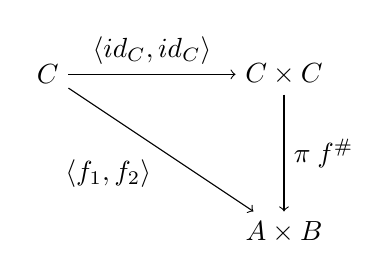
\begin{tikzpicture}
      \node (1) {$C$};
      \node[right of=1,xshift=2cm] (2) {$C \times C$};
      \node[below of=2,yshift=-1cm] (3) {$A \times B$};

      \draw[->] (1) -- node[above] {$\langle id_C, id_C \rangle$} (2);
      \draw[->] (1) -- node[below left] {$\langle f_1 , f_2 \rangle$} (3);
      \draw[->] (2) -- node[right] {$\pi~f^{\#}$} (3);
    \end{tikzpicture}
  \end{center}

  And the diagram for the counit is:
  \begin{center}
    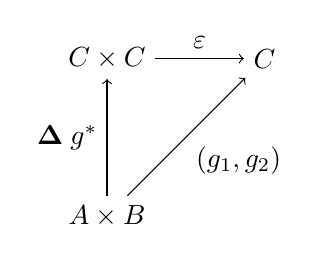
\begin{tikzpicture}
      \node (1) {$C \times C$};
      \node [below of=1,yshift=-1cm] (2) {$A \times B$};
      \node [right of=1,xshift=1cm] (3) {$C$};
      
      \draw[->] (2) -- node[left] {$\diagfun~g^*$} (1);
      \draw[->] (2) -- node[below right] {$(g_1, g_2)$} (3);
      \draw[->] (1) -- node[above] {$\varepsilon$} (3);
    \end{tikzpicture}
  \end{center}
  For $A \times B$ to match the definition of a product object it needs a unique arrow from any other object $X$ in $\cat$ that has arrows $f : X \rightarrow A$ and $g : X \rightarrow B$ and projection arrows to both $A$ and $B$.
  First, the unique arrow from an arbitrary object arises from the arrow $f^{\#}$ in the unit diagram.
  For an object $C$ with arrows $f_1$ and $f_2$ taking it to $A$ and $B$, respectively, the arrow $f^{\#}$ is uniquely determined to take the pair of objects $(C, C)$ to the pair of objects $(A,B)$.
  When mapped by the product functor, this gives the unique arrow into the product object $A \times B$.
  The projection arrows follow from the counit diagram because the counit $\varepsilon$ carries a pair formed from the product object $A \times B$ (that is, $(A \times B), (A \times B)$) to the pair of $A$ and $B$.
  Therefore $\varepsilon$ must be the pair of arrows $(\pi_1, \pi_2)$.
\end{enumerate}
\end{document}
